% ----------------------------------------------------
\begin{frame}
  \titlepage
\end{frame}
% ----------------------------------------------------
\note{}

% ----------------------------------------------------
\begin{frame}
\frametitle{Today's goals}
\centering

\begin{itemize}
\item Understand why spatial autocorrelation violates OLS assumptions
\item Diagnose spatial dependence: Moran's I on residuals and LM tests
\item Estimate the Spatial Error Model (SEM) and interpret $\lambda$
\item Estimate the Spatial Lag Model (SLM/SAR) and interpret $\rho$
\item Compute direct and indirect effects after SLM estimation
\item Understand estimation methods: ML, IV/2SLS, and why OLS fails
\item Choose between SEM, SLM, SDM, and extensions (SAC, SDEM)
\item Compare models: LR tests for nested models, AIC for non-nested
\end{itemize}

\end{frame}
% ----------------------------------------------------
\note{This session is the analytical companion to Session 7. Students already know how to work with spatial data in R and how to build spatial weights matrices with \texttt{spdep}. Today we ask: what do we do once we suspect that our regression residuals are spatially correlated? The answer involves two steps: diagnosis (Moran's I on residuals, LM tests) and cure (SEM or SLM or SDM). The conceptual distinction between SEM and SLM is the hardest part and deserves extra time. The lab component of this session will have students apply these models to a real dataset.}

% ====================================================
\section{Introduction to spatial dependence}
% ====================================================

% ----------------------------------------------------
\begin{frame}
\frametitle{A standard OLS regression}
\centering

\vspace{6pt}

$$y_i = \alpha + \mathbf{x}_i \boldsymbol{\beta} + \varepsilon_i$$

\vspace{12pt}

\begin{itemize}[<+->]
\item Classical assumption: $\varepsilon_i \sim \mathcal{N}(0, \sigma^2)$, independent across $i$
\vspace{8pt}
\item Spatial data violates this: observations are \textbf{not independent}
  \begin{itemize}
  \item Neighboring units share unmeasured common factors
  \item Outcomes may genuinely spill over across borders
  \end{itemize}
\vspace{8pt}
\item Consequence: OLS standard errors are \textbf{biased}
  \begin{itemize}
  \item Same problem as with clustered or heteroskedastic errors
  \item But the structure of dependence is explicitly \textit{geographic}
  \end{itemize}
\end{itemize}

\end{frame}
% ----------------------------------------------------
\note{Start with the familiar OLS setup and identify the violated assumption. The independence of errors assumption is what breaks down with spatial data. The analogy to panel data is useful: with panel data, residuals are correlated within units over time; with spatial data, residuals are correlated across neighboring units. Just as we use clustered standard errors for panel data, we need spatial corrections for geographic data. But in the spatial case, there are two fundamentally different reasons why residuals might be correlated, and the correct model depends on which mechanism is at work.}


% ----------------------------------------------------
\begin{frame}
\frametitle{Spatial weights: a brief recap}
\centering

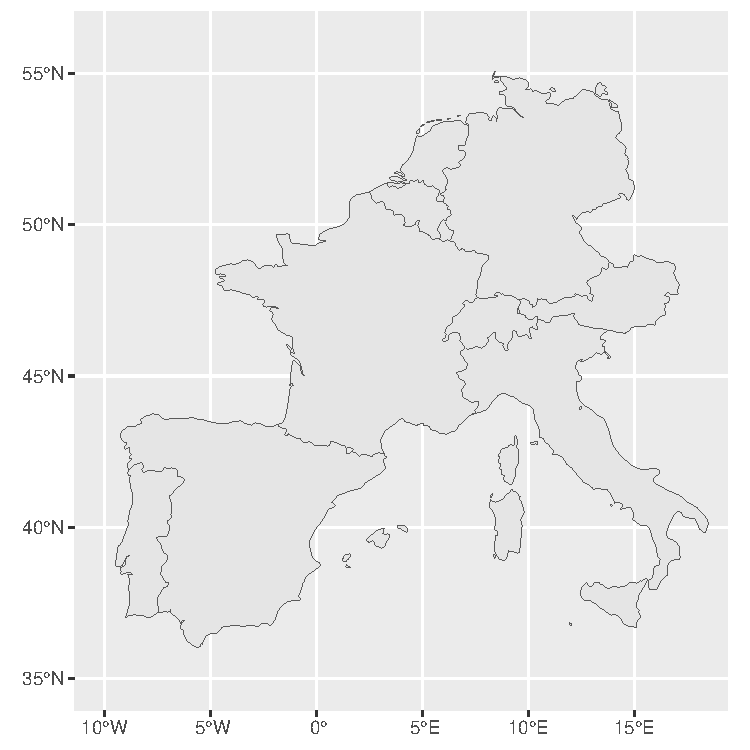
\includegraphics[height = .9\textheight]{../img/weurope}
  
\onslide<2->{
\begin{tikzpicture}[remember picture, overlay]
  \node[at = (current page.center), yshift = 0cm] (cover) {%
    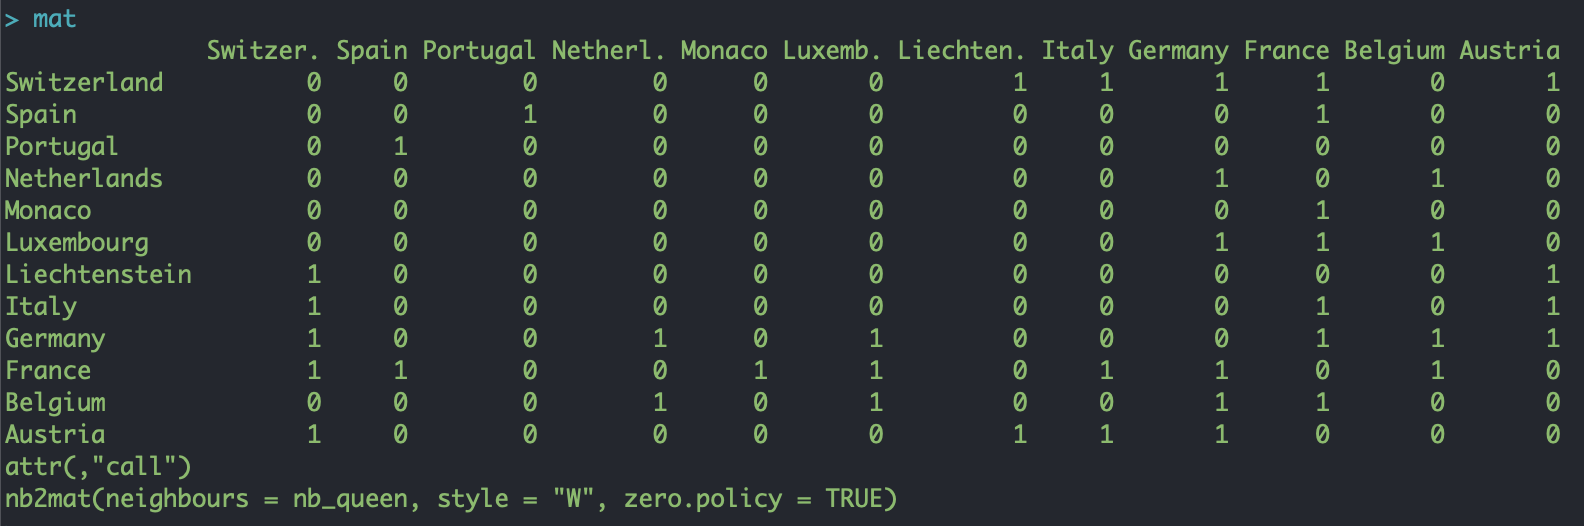
\includegraphics[keepaspectratio, width=.97\paperwidth]{../img/weuropemat1}};
\end{tikzpicture}}

\onslide<3->{
\begin{tikzpicture}[remember picture, overlay]
  \node[at = (current page.center), yshift = 0cm] (cover) {%
    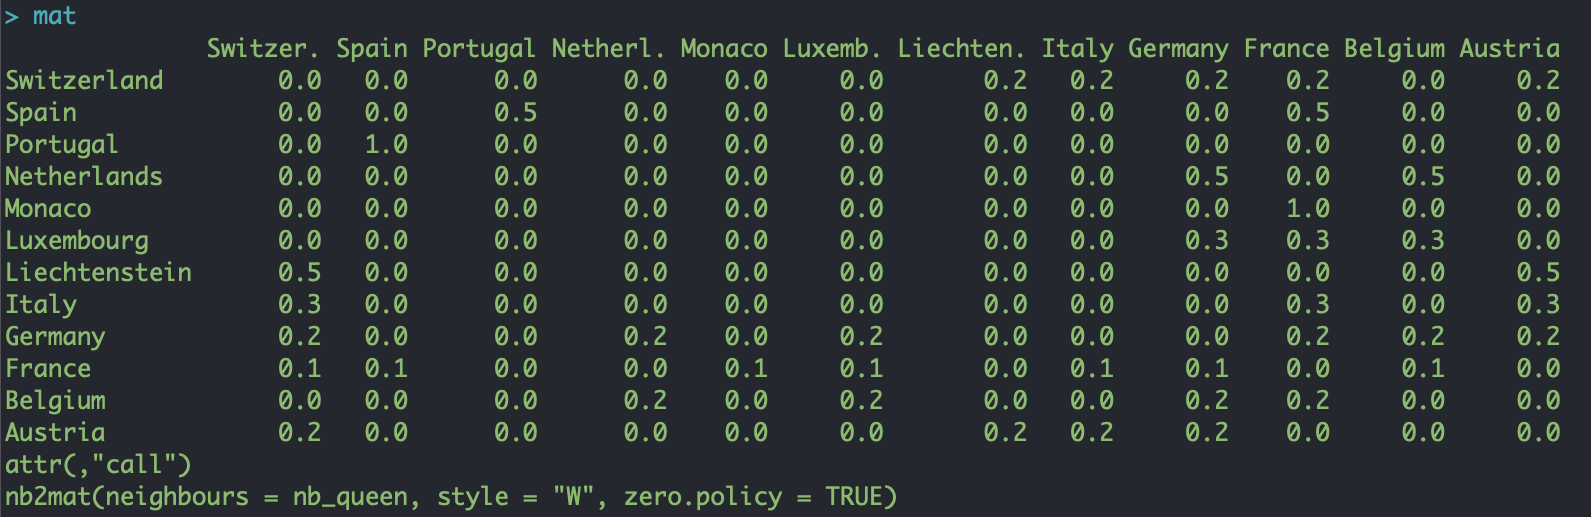
\includegraphics[keepaspectratio, width=.97\paperwidth]{../img/weuropemat2}};
\end{tikzpicture}}

\end{frame}
% ----------------------------------------------------
\note{...}

% ----------------------------------------------------
\begin{frame}
\frametitle{Spatial weights: a brief recap}
\centering

\begin{itemize}
    \item[] \textbf{Types of adjacency matrices} (with spatial data)
    \vspace{10pt}
    \item[1.]<2-> Based on \textbf{contiguity}
    \begin{itemize}
        \item Queen or rook {\small (or bishop, less common)}
    \end{itemize}
    \item[2.]<3-> Based on \textbf{distance}
    \begin{itemize}
        \item Distance threshold
        \item $k$-nearest neighbors (kNN)
    \end{itemize}
    \item[3.]<4-> Non-binary: weighted adjacency
    \begin{itemize}
        \item Based on distance (from border? from centroid? capital?), length of shared border, etc
    \end{itemize}
    \vspace{10pt}
    \item<5-> Conceptually, the same as a \textbf{network}, but just geographical
    \begin{itemize}
        \item<7-> e.g. difference with a network based on trade flows
        \item[]<8-> (but you could use \textbf{the same models on network data}!)
    \end{itemize}
\end{itemize}

\onslide<6>{
\begin{tikzpicture}[remember picture, overlay]
\fill[white] (current page.south west) rectangle (current page.north east);
  \node[at = (current page.center), yshift = 0cm] (cover) {%
    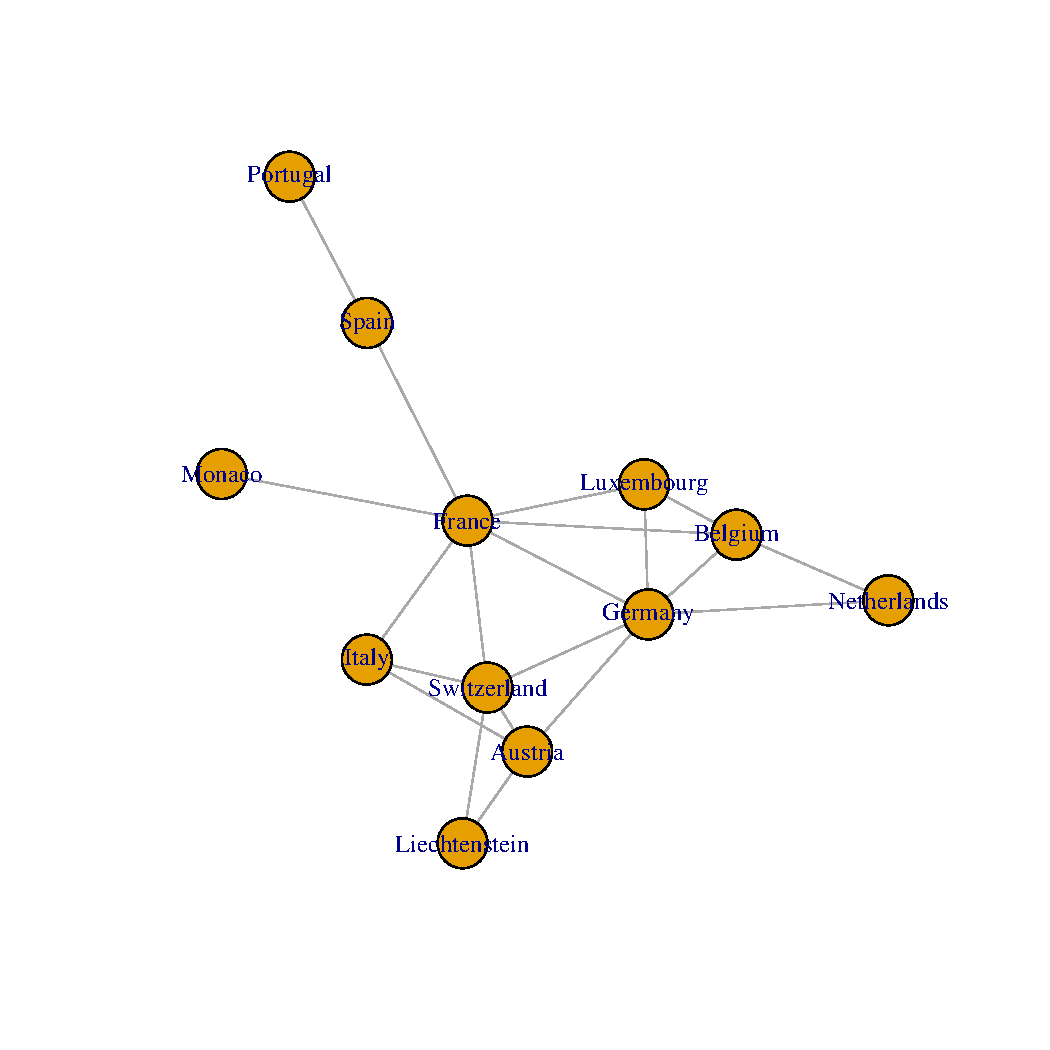
\includegraphics[keepaspectratio, width=.97\paperwidth]{../img/weuropemat_network}};
\end{tikzpicture}}

\end{frame}
% ----------------------------------------------------
\note{...}

% ----------------------------------------------------
\begin{frame}
\frametitle{Spatial weights: a brief recap}
\centering

\vspace{6pt}

\begin{columns}[T]
\begin{column}{0.55\textwidth}
  \begin{itemize}[<+->]
  \item $\mathbf{W}$: the $n \times n$ spatial weights matrix
  \item $w_{ij} > 0$ if $i$ and $j$ are neighbors, 0 otherwise
  \item (row-standardized matrix: rows sum to 1)
  \vspace{8pt}
  \item $\mathbf{W}\mathbf{y}$: the \textbf{spatial lag} of $\mathbf{y}$
    \begin{itemize}
    \item For each unit $i$: weighted average of neighbors' $y$
    \end{itemize}
  \vspace{8pt}
  \item In R: \texttt{poly2nb()} $\to$ \texttt{nb2listw()}
  \end{itemize}
\end{column}
\begin{column}{0.42\textwidth}
  \vspace{4pt}
  \begin{tikzpicture}[scale=0.85]
    \draw[fill=accent!10, draw=accent!50] (0,0) rectangle (1.4,1.4);
    \draw[fill=accent!10, draw=accent!50] (1.4,0) rectangle (2.8,1.4);
    \draw[fill=accent!10, draw=accent!50] (0,1.4) rectangle (1.4,2.8);
    \draw[fill=accent2!15, draw=accent2!60] (1.4,1.4) rectangle (2.8,2.8);
    \node[font=\footnotesize] at (0.7,0.7) {A};
    \node[font=\footnotesize] at (2.1,0.7) {B};
    \node[font=\footnotesize] at (0.7,2.1) {C};
    \node[font=\footnotesize, accent2] at (2.1,2.1) {\textbf{D}};
    \draw[->, thick, accent2] (2.1,2.1) -- (0.7,2.1);
    \draw[->, thick, accent2] (2.1,2.1) -- (2.1,0.7);
    \node[font=\scriptsize, asher, align=center] at (1.4,-0.4)
      {D's neighbors: B, C};
  \end{tikzpicture}
\end{column}
\end{columns}

\end{frame}
% ----------------------------------------------------
\note{Quick recap from Session 7 --- students already built weights matrices. The key concepts to refresh: the weights matrix $\mathbf{W}$ encodes the neighborhood structure; row standardization makes each row a proper weighted average; the spatial lag $\mathbf{W}\mathbf{y}$ is the average of neighbors' outcomes. This is the building block for all spatial models. If students are fuzzy on this, spend 2--3 minutes here before proceeding. For the models in this lecture, the weights matrix is always given: we do not estimate it, we choose it based on geographic contiguity or distance, then condition on it.}

% ----------------------------------------------------
\begin{frame}
\frametitle{Moran's I}
\centering

\vspace{6pt}

$$I = \frac{n}{\sum_{i}\sum_{j} w_{ij}} \cdot \frac{\sum_{i}\sum_{j} w_{ij}(y_i - \bar{y})(y_j - \bar{y})}{\sum_{i}(y_i - \bar{y})^2}$$

\vspace{10pt}

\begin{itemize}[<+->]
\item Ranges from $-1$ (perfect dispersion) to $+1$ (perfect clustering)
\item $I \approx 0$: no spatial autocorrelation (random)
\vspace{8pt}
\item Intuition: correlation between each unit's value and its \textbf{neighbors' values}
  \begin{itemize}
  \item High $I$: similar values cluster together (hot spots and cold spots)
  \item Low $I$: high and low values alternate (checkerboard pattern)
  \end{itemize}
\end{itemize}

\end{frame}
% ----------------------------------------------------
\note{Students saw Moran's I in Session 7 but may not have computed it themselves. Spend 2--3 minutes on the formula before moving on. The formula is a weighted correlation between $y_i$ and $\mathbf{W}y_i$ (the spatial lag). Under the null hypothesis of no spatial autocorrelation, the expected value of $I$ is $-1/(n-1) \approx 0$ for large $n$. A positive and significant $I$ means values cluster geographically: high values near high, low near low. This is the spatial analogue of serial correlation in time series. The key message for today: we are going to apply Moran's I not to the raw outcome $y$, but to the OLS \textit{residuals} --- that is where the problem shows up in regression analysis.}

% ----------------------------------------------------
\begin{frame}
\frametitle{The key diagnostic: Moran's I on residuals}
\centering

\vspace{6pt}

\begin{itemize}[<+->]
\item Run OLS first, compute residuals $\hat{\varepsilon}_i = y_i - \hat{y}_i$
\vspace{8pt}
\item Apply Moran's I to the \textbf{residuals}, not to $y$
  \begin{itemize}
  \item Spatial autocorrelation in $y$ alone may be explained by $\mathbf{x}$
  \item Autocorrelation in $\hat{\varepsilon}$ means the model has not removed the spatial structure
  \end{itemize}
\vspace{8pt}
\item In R:
\end{itemize}

\vspace{4pt}

\begin{block}{}
\texttt{ols\_fit = lm(y \textasciitilde{} x, data = mydata)}\\
\texttt{moran.test(residuals(ols\_fit), listw = my\_listw)}
\end{block}

\vspace{6pt}

{\small Significant Moran's I on residuals $\Rightarrow$ OLS is insufficient}

\end{frame}
% ----------------------------------------------------
\note{This is the first concrete step in the workflow. The Moran's I on residuals is a standard diagnostic in spatial econometrics. If the $p$-value is small (conventional threshold: $p < 0.05$), the null of no spatial autocorrelation is rejected and we should consider a spatial model. Note: a significant Moran's I tells us \textit{that} there is a problem but not \textit{which} model to use. For that, we need the Lagrange Multiplier tests covered in the next slide. The \texttt{moran.test()} function in \texttt{spdep} takes a numeric vector (the residuals) and a listw object. The function performs an analytical permutation test. An alternative is \texttt{moran.mc()} for a Monte Carlo permutation test.}

% ----------------------------------------------------
\begin{frame}
\frametitle{Two sources of spatial dependence}
\centering

\vspace{8pt}

\begin{tikzpicture}[
  box/.style={draw, rounded corners, minimum width=4.6cm, minimum height=1.1cm, align=center, font=\small},
  arrow/.style={->, thick, accent}
]
  \node[font=\small, align=center] (q) at (0, 3.4)
    {Moran's I on OLS residuals is significant \\ --- why?};
  \node[box, fill=accent!12]  (sem) at (-3.0, 1.8)
    {\textbf{Nuisance correlation}\\Unmeasured spatially\\correlated factors};
  \node[box, fill=accent2!12] (slm) at ( 3.0, 1.8)
    {\textbf{True spillover}\\Outcome in unit $i$\\affects neighbors $j$};
  \node[font=\small, accent]  (semm) at (-3.0, 0.2) {$\Rightarrow$ Spatial Error Model};
  \node[font=\small, accent2] (slmm) at ( 3.0, 0.2) {$\Rightarrow$ Spatial Lag Model};
  \draw[arrow] (q) -- (sem);
  \draw[arrow] (q) -- (slm);
\end{tikzpicture}

\vspace{8pt}
{\small\color{asher} Same symptom, different model}

\vspace{8pt}
Think about \textbf{your projects}: which mechanism is more plausible?

\end{frame}
% ----------------------------------------------------
\note{This is the central conceptual slide of the lecture. The two paths have the same observable symptom --- spatially correlated residuals --- but require fundamentally different model specifications. Nuisance correlation: your model is missing some variable that clusters geographically (historical culture, climate, infrastructure), so the residuals absorb that spatial structure. True spillover: the value of $y$ in one unit directly causes or influences $y$ in neighboring units (democracy diffusion, conflict contagion, economic agglomeration). The SEM captures the first; the SLM captures the second. The practical decision between them requires both statistical tests and substantive reasoning about the data-generating process. Return to this distinction throughout the lecture.}

% ----------------------------------------------------
\begin{frame}
\frametitle{LM tests: which model to choose?}
\centering

\vspace{6pt}

\begin{itemize}[<+->]
\item \textbf{LM tests} (Lagrange Multiplier): test for specific types of spatial dependence
\vspace{6pt}
\item Two tests, evaluated jointly:
  \begin{itemize}
  \item \textbf{LMerr}: tests for spatial error dependence ($\lambda \neq 0$)
  \item \textbf{LMlag}: tests for spatial lag dependence ($\rho \neq 0$)
  \end{itemize}
\vspace{6pt}
\item Robust versions: \textbf{RLMerr} and \textbf{RLMlag}
  \begin{itemize}
  \item Control for the presence of the other type of dependence
  \end{itemize}
\vspace{6pt}
\item In R:
\end{itemize}

\vspace{4pt}

\begin{block}{}
\texttt{lm.LMtests(ols\_fit, listw = my\_listw,}\\
\texttt{\hspace{12pt}test = c("LMerr", "LMlag", "RLMerr", "RLMlag"))}
\end{block}

\end{frame}
% ----------------------------------------------------
\note{The Anselin (1988) Lagrange Multiplier tests are the standard tool for choosing between SEM and SLM. Run them on the OLS object (not on a spatial model). The LM tests are computed from the OLS residuals without estimating the full spatial model, so they are fast. The decision rule: (1) if only LMerr is significant $\to$ SEM; (2) if only LMlag is significant $\to$ SLM; (3) if both are significant, look at RLMerr vs.\ RLMlag and choose the one with the higher test statistic. In practice, both are often significant, so the robust versions are usually what guides the decision. Tell students: the LM tests are a \textit{statistical} guide; the substantive question (nuisance vs. genuine spillover) should also inform the choice.}

% ----------------------------------------------------
\begin{frame}
\frametitle{LM decision rule}
\centering

\vspace{10pt}

\begin{tikzpicture}[
  dec/.style={draw, fill=accent!15, minimum width=3.4cm, minimum height=0.85cm, align=center, font=\small},
  box/.style={draw, rounded corners, fill=accent2!10, minimum width=2.8cm, minimum height=0.8cm, align=center, font=\small},
  arrow/.style={->, thick, asher}
]
  \node[dec] (moran) at (0, 3.5) {Moran's I on\\residuals significant?};
  \node[font=\small, text=asher] (ok) at (-4.0, 3.5) {Stop: OLS is fine};
  \node[dec] (lm) at (0, 1.8) {LMerr or LMlag\\significant?};
  \node[box] (sem) at (-3.2, 0.2) {SEM\\(or SDM)};
  \node[box] (slm) at ( 3.2, 0.2) {SLM\\(or SDM)};
  \node[box] (sdm) at (0, 0.2) {Both: compare\\RLM tests};
  \draw[arrow] (moran) -- node[font=\scriptsize, text=accent2, midway, above]{No} (ok);
  \draw[arrow] (moran) -- node[font=\scriptsize, text=accent, midway, right]{Yes} (lm);
  \draw[arrow] (lm) -- node[font=\scriptsize, text=accent, midway, above left]{LMerr only} (sem);
  \draw[arrow] (lm) -- node[font=\scriptsize, text=accent, midway, above right]{LMlag only} (slm);
  \draw[arrow] (lm) -- node[font=\scriptsize, text=accent, midway, right]{Both} (sdm);
\end{tikzpicture}

\end{frame}
% ----------------------------------------------------
\note{This decision tree summarizes the diagnostic workflow. Walk through it step by step: first Moran's I tells us whether there is a problem at all; if yes, the LM tests guide model selection. In applied work, students will often find that both LMerr and LMlag are significant --- this is the common case with real spatial data. When that happens, use the robust versions (RLMerr, RLMlag) and choose the model corresponding to the larger and more significant test. The SDM (Spatial Durbin Model, covered at the end) nests both SEM and SLM and is a conservative choice when both tests are significant. Note: this is a statistical decision rule; always complement it with theory about whether spatial diffusion is a plausible mechanism in your setting.}

% ====================================================
\section{The Spatial Error Model (SEM)}
% ====================================================

% ----------------------------------------------------
\begin{frame}
\frametitle{SEM: the model}
\centering

\vspace{8pt}

\begin{block}{Spatial Error Model}
$$\mathbf{y} = \mathbf{X}\boldsymbol{\beta} + \mathbf{u}$$
$$\mathbf{u} = \lambda \mathbf{W}\mathbf{u} + \boldsymbol{\varepsilon}, \quad \boldsymbol{\varepsilon} \sim \mathcal{N}(\mathbf{0}, \sigma^2 \mathbf{I})$$
\end{block}

\vspace{12pt}

\begin{itemize}[<+->]
\item $\mathbf{W}$: spatial weights matrix
\item $\lambda$ (lambda): spatial autocorrelation in the \textbf{error term}
  \begin{itemize}
  \item $\lambda = 0$: back to standard OLS
  \item $\lambda > 0$: positive spatial autocorrelation in errors
  \end{itemize}
\vspace{6pt}
\item $\boldsymbol{\beta}$: same interpretation as OLS
\item The spatial structure is in the \textbf{residuals}, not in the outcome
\end{itemize}

\end{frame}
% ----------------------------------------------------
\note{The SEM has two equations. The first is the familiar regression equation: outcome is a linear function of covariates plus a composite error $\mathbf{u}$. The second equation describes how the error is generated: the error at unit $i$ is a function of the errors at neighboring units (via $\lambda\mathbf{W}\mathbf{u}$) plus an independent shock $\varepsilon_i$. Solving the second equation for $\mathbf{u}$ gives: $\mathbf{u} = (I - \lambda W)^{-1}\varepsilon$, which is a non-diagonal covariance matrix. This is why OLS is inefficient: it assumes diagonal covariance. The key insight: $\lambda$ is a \textit{nuisance parameter}. We estimate it to get correct SEs and efficient estimates of $\beta$, but $\beta$ retains its standard OLS interpretation. There is no substantive spillover story in the SEM.}

% ----------------------------------------------------
\begin{frame}
\frametitle{SEM: substantive interpretation}
\centering

\vspace{8pt}

\begin{itemize}[<+->]
\item The SEM says: \textbf{unmeasured factors} that affect $y$ are geographically clustered
\vspace{8pt}
\item Examples:
  \begin{itemize}
  \item Country democracy regressed on GDP: unmeasured historical institutions cluster geographically
  \item Municipal health outcomes: regional infrastructure and public goods affect nearby areas
  \item Conflict event density: unobserved security capacity clusters across provinces
  \end{itemize}
\vspace{8pt}
\item $\lambda \neq 0$ does \textbf{not} mean $y$ affects neighbors' $y$
  \begin{itemize}
  \item It means the residuals are spatially structured
  \end{itemize}
\vspace{8pt}
\item Fix: correct SEs and improve efficiency --- not model substantive spillover
\end{itemize}

\end{frame}
% ----------------------------------------------------
\note{Ground the SEM in substantive examples students will recognize. The democracy example: Acemoglu, Johnson and Robinson use colonial history as an instrument --- but colonial legacies are geographically clustered. If you regress democracy on GDP without controlling for colonial history, the residuals will cluster geographically. The SEM is the right model because the spatial dependence is in omitted variables, not in a democracy-contagion mechanism. Stress: the SEM is primarily a correction, not an explanation. The coefficient on $\lambda$ itself is rarely the quantity of interest; the goal is to get unbiased and efficient estimates of $\beta$. If you have a strong prior that democracy \textit{does} spread across borders, the SLM (next section) is the right choice.}

% ----------------------------------------------------
\begin{frame}
\frametitle{SEM in R}
\centering

\vspace{6pt}

\begin{itemize}
\item[] \texttt{library(spatialreg) \# or spdep}
\item[] \phantom{x}
\item[] \texttt{\# Fit Spatial Error Model}
\item[] \texttt{sem\_fit = errorsarlm(y \textasciitilde{} x1 + x2,}
\item[] \texttt{\hspace{20pt}data = mydata,}
\item[] \texttt{\hspace{20pt}listw = my\_listw,}
\item[] \texttt{\hspace{20pt}zero.policy = TRUE)}
\item[] \phantom{x}
\item[] \texttt{summary(sem\_fit)}
\end{itemize}

\vspace{8pt}

\begin{itemize}[<+->]
\item \texttt{errorsarlm()}: maximum likelihood estimation of SEM
\item \texttt{zero.policy = TRUE}: allow units with no neighbors
\item Key output: $\hat{\lambda}$ and its significance; $\hat{\boldsymbol{\beta}}$ interpreted as OLS
\end{itemize}

\end{frame}
% ----------------------------------------------------
\note{The function name \texttt{errorsarlm} is mnemonic for ``error spatial autoregressive linear model.'' It lives in both \texttt{spdep} (older, will be deprecated) and \texttt{spatialreg} (the modern fork). Tell students: load \texttt{spatialreg} explicitly to avoid namespace conflicts. The \texttt{zero.policy} argument handles units with no neighbors in the weights matrix (e.g., islands); setting it to \texttt{TRUE} allows the function to continue rather than throwing an error. The \texttt{summary()} output includes: the $\hat{\lambda}$ coefficient with SE and $p$-value, the regression coefficients $\hat{\beta}$, the log-likelihood, and model fit statistics (AIC, BIC). Tell students: if $\hat{\lambda}$ is not statistically significant, the SEM collapses to OLS and there was no need for the spatial correction.}

% ----------------------------------------------------
\begin{frame}
\frametitle{SEM: reading the output}
\centering

\vspace{4pt}

{\footnotesize
\begin{tabular}{lcccc}
\hline
 & \textbf{Estimate} & \textbf{Std. Error} & \textbf{$z$-value} & \textbf{$p$-value} \\
\hline
(Intercept)     & $-2.14$ & $0.48$ & $-4.45$ & $< 0.001$ \\
\texttt{gdp\_pc}  & $\phantom{-}0.63$ & $0.07$ & $\phantom{-}9.11$ & $< 0.001$ \\
\texttt{pop\_l}   & $\phantom{-}0.18$ & $0.05$ & $\phantom{-}3.37$ & $0.001$ \\
\hline
$\lambda$ (Lambda) & $\phantom{-}0.54$ & $0.09$ & $\phantom{-}5.80$ & $< 0.001$ \\
\hline
\end{tabular}
}

\vspace{10pt}

\begin{itemize}[<+->]
\item $\hat{\lambda} = 0.54$: strong positive spatial autocorrelation in errors
\item $\boldsymbol{\hat{\beta}}$: interpreted exactly as in OLS
\item Compare with OLS: coefficients may shift, SEs typically change
\item Use AIC/LR test to confirm SEM improves on OLS
\end{itemize}

\end{frame}
% ----------------------------------------------------
\note{Walk through a realistic output table. The $\hat{\lambda}$ appears at the bottom of the output, clearly labeled. A value of 0.54 indicates strong spatial autocorrelation in the error term --- errors in neighboring units are positively correlated. The $\beta$ coefficients are interpreted exactly as in OLS: a one-unit increase in \texttt{gdp\_pc} is associated with a 0.63-unit increase in $y$, holding other variables constant. Remind students: if the SEM $\hat{\beta}$ differs noticeably from the OLS $\hat{\beta}$, it suggests the original OLS estimate was affected by spatial confounding. A likelihood-ratio (LR) test against the restricted OLS model --- available via \texttt{anova(sem\_fit, ols\_fit)} --- formally tests whether the SEM is a statistically significant improvement.}

% ====================================================
\section{The Spatial Lag Model (SLM/SAR)}
% ====================================================

% ----------------------------------------------------
\begin{frame}
\frametitle{SLM: the model}
\centering

\vspace{8pt}

\begin{block}{Spatial Lag Model (SLM / SAR)}
$$\mathbf{y} = \rho \mathbf{W}\mathbf{y} + \mathbf{X}\boldsymbol{\beta} + \boldsymbol{\varepsilon}, \quad \boldsymbol{\varepsilon} \sim \mathcal{N}(\mathbf{0}, \sigma^2 \mathbf{I})$$
\end{block}

\vspace{12pt}

\begin{itemize}[<+->]
\item $\rho$ (rho): spatial autoregressive parameter on the \textbf{lagged outcome}
  \begin{itemize}
  \item $\rho = 0$: standard OLS
  \item $\rho > 0$: positive spatial diffusion (clustering in $y$)
  \end{itemize}
\vspace{6pt}
\item $\mathbf{W}\mathbf{y}$: the spatial lag --- average of neighbors' $y$
\vspace{6pt}
\item \alert{Key difference from SEM}: the spatial lag is on the \textbf{outcome}, not the error
\item $y_i$ is partly determined by its neighbors' $y_j$
\end{itemize}

\end{frame}
% ----------------------------------------------------
\note{The SLM adds the spatially lagged dependent variable $\mathbf{W}\mathbf{y}$ as a regressor. This is the key structural difference from SEM: $\rho$ captures genuine spillover, not nuisance correlation. The endogeneity problem is immediate: $\mathbf{W}\mathbf{y}$ is correlated with $\varepsilon$ (because neighboring $y_j$ depends on neighboring $\varepsilon_j$, which feeds back through the weights matrix). OLS applied to this equation would give biased estimates of $\rho$. This is why the SLM is estimated by maximum likelihood (or instrumental variables), not OLS. The equilibrium interpretation: in the SLM, $y_i$ affects $y_j$, which affects $y_k$, and so on until the system reaches equilibrium. This feedback loop is what makes direct and indirect effects differ (Section 6).}

% ----------------------------------------------------
\begin{frame}
\frametitle{SLM: substantive interpretation}
\centering

\vspace{8pt}

\begin{itemize}[<+->]
\item The SLM says: your outcome \textbf{depends on neighbors' outcomes}
\vspace{8pt}
\item Examples of genuine spatial diffusion:
  \begin{itemize}
  \item \textbf{Democracy}: a country becomes more democratic partly because its neighbors are democratic
  \item \textbf{Economic development}: city growth spills over to nearby cities (agglomeration)
  \item \textbf{Conflict}: violence in one district raises conflict risk in adjacent districts
  \item \textbf{Policy adoption}: states imitate neighboring states' welfare policies
  \end{itemize}
\vspace{8pt}
\item $\rho > 0$: spatial diffusion (neighbors' high $y$ raises your $y$)
\vspace{8pt}
\item \alert{Warning}: $\boldsymbol{\hat{\beta}}$ from SLM is \textbf{not} the marginal effect of $\mathbf{x}$ on $y$
\end{itemize}

\end{frame}
% ----------------------------------------------------
\note{The substantive examples are crucial for helping students see when to choose SLM over SEM. Democracy diffusion is a real research agenda (Gleditsch and Ward 2006): countries with democratic neighbors are more likely to democratize. Economic geography research on agglomeration effects (Krugman 1991): firms and workers concentrate in already-large cities partly because others have done the same. Conflict diffusion (Buhaug and Gleditsch 2008): civil war in country A increases the risk of civil war in neighboring country B, through refugee flows, arms trafficking, or spillover of fighting. In all these cases, the DGP has $y_i$ causally affecting $y_j$. The alert at the bottom is the key warning for the next section: unlike OLS or SEM, the coefficient $\hat{\beta}$ in the SLM is not the marginal effect of $x$ on $y$.}

% ----------------------------------------------------
\begin{frame}
\frametitle{SLM in R}
\centering

\vspace{6pt}

\begin{itemize}
\item[] \texttt{library(spatialreg)}
\item[] \phantom{x}
\item[] \texttt{\# Fit Spatial Lag Model}
\item[] \texttt{slm\_fit = lagsarlm(y \textasciitilde{} x1 + x2,}
\item[] \texttt{\hspace{20pt}data = mydata,}
\item[] \texttt{\hspace{20pt}listw = my\_listw,}
\item[] \texttt{\hspace{20pt}zero.policy = TRUE)}
\item[] \phantom{x}
\item[] \texttt{summary(slm\_fit)}
\end{itemize}

\vspace{8pt}

\begin{itemize}[<+->]
\item \texttt{lagsarlm()}: ML estimation of SLM
\item Key output: $\hat{\rho}$ and its significance; $\hat{\boldsymbol{\beta}}$ (not marginal effects!)
\item \alert{Do not interpret $\hat{\boldsymbol{\beta}}$ directly} --- use \texttt{impacts()} instead
\end{itemize}

\end{frame}
% ----------------------------------------------------
\note{The function \texttt{lagsarlm} is the SLM counterpart to \texttt{errorsarlm}. The syntax is nearly identical: swap function name, same \texttt{listw} argument. Students will notice the output also looks similar to SEM output: a $\hat{\rho}$ coefficient replaces $\hat{\lambda}$, and $\hat{\beta}$ coefficients appear for the covariates. The critical warning is that the $\hat{\beta}$ coefficients in the SLM output are not marginal effects and should not be interpreted as such. They represent the direct effect on $y_i$ holding neighbors' $y$ constant --- but that counterfactual is not realistic, because changing $x_i$ changes $y_i$, which changes neighbors' $\mathbf{W}y$, which changes $y_i$ again. The correct procedure is \texttt{impacts()}, which accounts for this feedback. Tell students: always use \texttt{impacts()} for inference after estimating a SLM.}

% ----------------------------------------------------
\begin{frame}
\frametitle{SLM: reading the output}
\centering

\vspace{4pt}

{\footnotesize
\begin{tabular}{lcccc}
\hline
 & \textbf{Estimate} & \textbf{Std. Error} & \textbf{$z$-value} & \textbf{$p$-value} \\
\hline
(Intercept)     & $-1.87$ & $0.52$ & $-3.59$ & $< 0.001$ \\
\texttt{gdp\_pc}  & $\phantom{-}0.51$ & $0.08$ & $\phantom{-}6.29$ & $< 0.001$ \\
\texttt{pop\_l}   & $\phantom{-}0.14$ & $0.05$ & $\phantom{-}2.85$ & $0.004$ \\
\hline
$\rho$ (Rho)    & $\phantom{-}0.48$ & $0.10$ & $\phantom{-}4.90$ & $< 0.001$ \\
\hline
\end{tabular}
}

\vspace{10pt}

\begin{itemize}[<+->]
\item $\hat{\rho} = 0.48$: strong positive spatial diffusion in $y$
\item $\hat{\boldsymbol{\beta}}$ coefficients appear in output \textbf{but are not marginal effects}
\item Marginal effects are obtained via \texttt{impacts(slm\_fit, listw = my\_listw)}
\end{itemize}

\end{frame}
% ----------------------------------------------------
\note{Walk through this output table. The structure mirrors the SEM output: $\hat{\rho}$ at the bottom, $\hat{\beta}$ for each covariate above. The value $\hat{\rho} = 0.48$ is substantively meaningful: after controlling for GDP and population, each unit's $y$ is on average 48\% as large as the average of its neighbors' $y$. But notice the warning: the $\hat{\beta}$ for \texttt{gdp\_pc} is 0.51, not 0.63 as in the SEM. Which is the marginal effect? Neither the raw $\hat{\beta}$ nor the SEM coefficient --- we need the \texttt{impacts()} function, which accounts for the equilibrium feedback loop. This is the topic of the next section.}

% ====================================================
\section{Direct and Indirect Effects}
% ====================================================

% ----------------------------------------------------
\begin{transitionframe}
Changing $x_i$ creates a ripple through the network.\\[8pt]
The coefficient $\hat{\boldsymbol{\beta}}$ is not the marginal effect.
\end{transitionframe}
% ----------------------------------------------------
\note{Use this transition to signal the conceptual shift: we are moving from model estimation to equilibrium interpretation. Key idea to plant in students' minds: in the SLM, a change in $x_i$ raises $y_i$, which through the spatial lag raises neighbors' $y_j$, which in turn raises $y_i$ again (feedback), and so on until equilibrium. The total effect is therefore larger than the coefficient, and neighboring units are also affected.}

% ----------------------------------------------------
\begin{frame}
\frametitle{Why $\hat{\boldsymbol{\beta}}$ is not the marginal effect}
\centering

Solving the SLM for $\mathbf{y}$:

$\mathbf{y} = \rho\mathbf{W}\mathbf{y} + \mathbf{X}\boldsymbol{\beta} + \boldsymbol{\varepsilon}$

$(\mathbf{I} - \rho\mathbf{W})\mathbf{y} = \mathbf{X}\boldsymbol{\beta} + \boldsymbol{\varepsilon}$

$\mathbf{y} = \underbrace{(\mathbf{I} - \rho\mathbf{W})^{-1}}_{\mathbf{B}} (\mathbf{X}\boldsymbol{\beta} + \boldsymbol{\varepsilon})$

\vspace{10pt}

\begin{itemize}[<+->]
\item $\mathbf{B} = (\mathbf{I} - \rho\mathbf{W})^{-1}$: the \textbf{equilibrium effects matrix}
\item A change in $x_i$ propagates through $\mathbf{B}$: affects $y_i$ \textbf{and} all $y_j$
\item $\partial y_i / \partial x_i \neq \hat{\beta}$
\vspace{8pt}
\item \textbf{Question:} if you change $x_i$, how many units in the network are eventually affected?
\end{itemize}

\end{frame}
% ----------------------------------------------------
\note{This is the most technical slide in the lecture but the derivation is straightforward algebra. Start with the SLM equation, move $\rho\mathbf{W}\mathbf{y}$ to the left side, factor out $(\mathbf{I} - \rho\mathbf{W})$, and invert. The matrix $\mathbf{B} = (\mathbf{I} - \rho\mathbf{W})^{-1}$ is not the identity matrix (unless $\rho = 0$); it encodes the equilibrium propagation of shocks through the spatial network. The $(i,j)$ element of $\mathbf{B}$ tells you how much a unit change in $x_k$ for unit $j$ affects $y_i$, after all spatial feedback has played out. The diagonal elements give the direct effects; the off-diagonal elements give the indirect (spillover) effects. Because $\mathbf{B}$ is typically non-diagonal and all elements depend on $\rho$ and $\mathbf{W}$, the marginal effects are different for each observation. In practice we report the average, which is what \texttt{impacts()} computes.}

% ----------------------------------------------------
\begin{frame}
\frametitle{Direct, indirect, and total effects}
\centering

\vspace{6pt}

\begin{tikzpicture}[
  box/.style={draw, rounded corners, minimum width=3.8cm, minimum height=0.9cm, align=center, font=\small},
  arrow/.style={->, thick, accent}
]
  \node[box, fill=accent!12]  (dir) at (-3.2, 0) {\textbf{Direct effect}\\Effect of $x_i$ on $y_i$\\(avg.\ diagonal of $\mathbf{B}\beta_k$)};
  \node[box, fill=accent2!12] (ind) at ( 3.2, 0) {\textbf{Indirect effect}\\Effect of $x_i$ on $y_j$, $j \neq i$\\(avg.\ off-diagonal)};
  \node[box, fill=asher!10]   (tot) at (0, -1.9) {\textbf{Total effect}\\ Direct + Indirect};
  \draw[arrow] (dir) -- (tot);
  \draw[arrow] (ind) -- (tot);
\end{tikzpicture}

\vspace{10pt}

\begin{itemize}[<+->]
\item Direct $\approx \hat{\beta}_k$ but slightly larger due to own-unit feedback
\item Indirect: captures spatial spillover --- ignored by OLS and SEM
\item Total: the full equilibrium effect of a uniform shock to $x_k$
\end{itemize}

\end{frame}
% ----------------------------------------------------
\note{The three-way decomposition is the key practical output from a SLM. The direct effect is the average effect of a unit's own $x_k$ on its own $y$ --- it is slightly larger than $\hat{\beta}_k$ because of own-unit feedback through the weights matrix (a change in $x_i$ changes $y_i$, which changes $\mathbf{W}y_i$, which changes $y_i$ again). The indirect effect (also called the spillover effect or the global effect) measures how a unit's $x_k$ affects all other units' outcomes. This is the novel quantity that the SLM estimates and that OLS/SEM miss entirely. The total effect is the sum: it answers the question ``if I uniformly increase $x_k$ by one unit for all units, what is the average change in $y$?'' This is the policy-relevant quantity for spatially connected units.}

% ----------------------------------------------------
\begin{frame}
\frametitle{Computing impacts in R}
\centering

\vspace{4pt}

\begin{itemize}
\item[] \texttt{\# Direct, indirect, total effects}
\item[] \texttt{imp = impacts(slm\_fit, listw = my\_listw)}
\item[] \texttt{summary(imp, zstats = TRUE)}
\item[] \phantom{x}
\item[] \texttt{\#\# Impact measures (lag, exact):}
\item[] \texttt{\#\#\hspace{10pt}Direct\hspace{4pt}Indirect\hspace{4pt}Total}
\item[] \texttt{\# gdp\_pc\hspace{4pt}0.574\hspace{12pt}0.531\hspace{8pt}1.105}
\item[] \texttt{\# pop\_l\hspace{8pt}0.161\hspace{12pt}0.149\hspace{8pt}0.310}
\end{itemize}

\vspace{8pt}

\begin{itemize}[<+->]
\item \textbf{Direct} (\texttt{gdp\_pc}): 0.574 --- unit's own GDP raises own $y$ by 0.574
\item \textbf{Indirect}: 0.531 --- unit's GDP raises neighbors' $y$ by 0.531 on average
\item \textbf{Total}: 1.105 --- full equilibrium effect ($> \hat{\beta}_k = 0.51$)
\item Use \texttt{zstats = TRUE} to get $z$-statistics and $p$-values
\end{itemize}

\end{frame}
% ----------------------------------------------------
\note{Walk through the \texttt{impacts()} output in detail. The function takes the estimated model object and the weights matrix (needed to compute $\mathbf{B}$). The output table has three columns (Direct, Indirect, Total) and one row per covariate. The numbers in this example show: (1) the direct effect (0.574) is slightly larger than $\hat{\beta}_k$ (0.51 from the SLM output) due to feedback; (2) the indirect effect (0.531) is substantial --- roughly equal to the direct effect; (3) the total effect (1.105) is more than double $\hat{\beta}_k$. This means ignoring spatial spillover would severely underestimate the impact of GDP on $y$. The \texttt{zstats = TRUE} argument includes asymptotic standard errors and $z$-statistics computed by simulation. Always report the impacts table in papers that use SLM.}

% % ----------------------------------------------------
% \begin{frame}
% \frametitle{Spatial feedback: intuition}
% \centering

% \vspace{8pt}

% \begin{tikzpicture}[scale=0.9]
%   % Units
%   \node[draw, circle, fill=accent!15, minimum size=1.0cm, font=\small] (i)  at (0, 0)   {$i$};
%   \node[draw, circle, fill=accent!8,  minimum size=0.8cm, font=\small] (j1) at (-2.5, 1.2) {$j_1$};
%   \node[draw, circle, fill=accent!8,  minimum size=0.8cm, font=\small] (j2) at ( 2.5, 1.2) {$j_2$};
%   \node[draw, circle, fill=accent!8,  minimum size=0.8cm, font=\small] (j3) at (0,   -1.8) {$j_3$};
%   % Arrows: i to neighbors
%   \draw[->, thick, accent2] (i)  -- node[above left, font=\scriptsize]{$\rho w_{j_1 i}$} (j1);
%   \draw[->, thick, accent2] (i)  -- node[above right, font=\scriptsize]{$\rho w_{j_2 i}$} (j2);
%   \draw[->, thick, accent2] (i)  -- node[right, font=\scriptsize]{$\rho w_{j_3 i}$} (j3);
%   % x_i shock label
%   \node[font=\small, asher, align=center] at (0, 1.0) {$\Delta x_i \uparrow$\\$\Downarrow$\\$\Delta y_i \uparrow$};
% \end{tikzpicture}

% \vspace{6pt}
% {\small $\Delta y_i \uparrow$ $\Rightarrow$ $\Delta(\mathbf{W}\mathbf{y})_j \uparrow$ $\Rightarrow$ $\Delta y_j \uparrow$ for all neighbors $j$, then ripples further}

% \end{frame}
% % ----------------------------------------------------
% \note{Visual intuition for spatial feedback. A shock to $x_i$ raises $y_i$ (direct effect). Because unit $i$ is in neighbors' spatial lag, their $\mathbf{W}y$ rises, which raises their $y_j$ (first-order indirect effect). But now $i$ also has those $j$ units as neighbors, so $\mathbf{W}y_i$ rises further, raising $y_i$ again (own-unit feedback). This continues until the system reaches equilibrium. For large $\rho$ and densely connected networks, these feedback effects can be substantial --- the total effect far exceeds the direct effect. This is why simply ignoring $\rho$ and interpreting $\hat{\beta}$ directly leads to large underestimates of the full policy impact. The network structure captured by $\mathbf{W}$ determines how far and how fast shocks propagate.}

% ====================================================
\section{The Spatial Durbin Model (SDM)}
% ====================================================

% ----------------------------------------------------
\begin{frame}
\frametitle{SDM: extending the SLM}
\centering

\vspace{8pt}

\begin{block}{Spatial Durbin Model}
$$\mathbf{y} = \rho \mathbf{W}\mathbf{y} + \mathbf{X}\boldsymbol{\beta} + \mathbf{W}\mathbf{X}\boldsymbol{\theta} + \boldsymbol{\varepsilon}$$
\end{block}

\vspace{10pt}

\begin{itemize}[<+->]
\item Adds spatially lagged covariates $\mathbf{W}\mathbf{X}\boldsymbol{\theta}$ to the SLM
\item $\theta_k$: effect of \textbf{neighbors' $x_k$} on unit $i$'s $y$
\vspace{6pt}
\item Most flexible model:
  \begin{itemize}
  \item SLM is nested ($\boldsymbol{\theta} = 0$)
  \item SEM is nested ($\boldsymbol{\theta} = -\rho\boldsymbol{\beta}$)
  \end{itemize}
\vspace{6pt}
\item LeSage \& Pace (2009): SDM is often preferred as a conservative default
\end{itemize}

\end{frame}
% ----------------------------------------------------
\note{The SDM nests both the SEM and the SLM as special cases, making it the most general of the three models. Adding $\mathbf{W}\mathbf{X}\boldsymbol{\theta}$ allows neighbors' covariates to directly affect unit $i$'s outcome, in addition to the spatial lag of $y$. Substantive example: in a trade model, both a country's own GDP ($\mathbf{X}\boldsymbol{\beta}$) and its neighbors' GDP ($\mathbf{W}\mathbf{X}\boldsymbol{\theta}$) may affect trade flows, along with spatial diffusion in the dependent variable ($\rho\mathbf{W}\mathbf{y}$). The SDM is often recommended as a default when both LM tests are significant, because it reduces the risk of model misspecification. The cost is more parameters to estimate. Note: $\boldsymbol{\hat{\beta}}$ and $\boldsymbol{\hat{\theta}}$ from SDM are also not marginal effects --- you still need \texttt{impacts()} for correct inference.}

% ----------------------------------------------------
\begin{frame}
\frametitle{SDM in R and when to use it}
\centering

\vspace{4pt}

\begin{itemize}
\item[] \texttt{\# Spatial Durbin Model}
\item[] \texttt{sdm\_fit = lagsarlm(y \textasciitilde{} x,}
\item[] \texttt{\hspace{20pt}data = mydata,}
\item[] \texttt{\hspace{20pt}listw = my\_listw,}
\item[] \texttt{\hspace{20pt}Durbin = TRUE,}
\item[] \texttt{\hspace{20pt}zero.policy = TRUE)}
\item[] \phantom{x}
\item[] \texttt{\# Direct, indirect, total as usual}
\item[] \texttt{impacts(sdm\_fit, listw = my\_listw)}
\end{itemize}

\vspace{8pt}

\begin{itemize}[<+->]
\item \texttt{Durbin = TRUE}: adds $\mathbf{W}\mathbf{X}$ to \texttt{lagsarlm()}
\item Use SDM when: neighbors' $\mathbf{x}$ plausibly affects $y$
\item Also useful as robustness check for SLM estimates
\end{itemize}

\end{frame}
% ----------------------------------------------------
\note{The SDM is fit with the same function as the SLM (\texttt{lagsarlm}) by adding \texttt{type = "mixed"}. This instructs the function to also include all spatially lagged covariates automatically. The output will include $\hat{\rho}$, $\hat{\beta}$ for own-unit covariates, and $\hat{\theta}$ (labeled \texttt{lag.x1}, \texttt{lag.x2}, etc.) for the spatially lagged covariates. As with the SLM, do not interpret these coefficients directly --- use \texttt{impacts()} for the correct direct, indirect, and total effects. When to use SDM: (1) both LM tests significant; (2) substantive theory suggests neighbors' $x$ matters; (3) as a robustness check to confirm SLM results are not sensitive to excluding $\mathbf{W}\mathbf{X}$. LeSage and Pace (2009) argue the SDM is generally preferable to SEM for applied research because it allows more flexible spillover patterns.}

% ====================================================
\section{Estimation Methods}
% ====================================================

% ----------------------------------------------------
\begin{frame}
\frametitle{How are these models estimated?}
\centering

\vspace{6pt}

{\footnotesize
\begin{tabular}{p{1.8cm}p{2.5cm}p{5.0cm}}
\hline
\textbf{Model} & \textbf{Estimation} & \textbf{Why not OLS?} \\
\hline
OLS        & OLS                & Baseline: valid if no spatial dependence \\[4pt]
SEM        & ML                 & OLS is unbiased but \textbf{inefficient}; SEs are wrong \\[4pt]
SLM        & ML (or IV/2SLS)    & $\mathbf{W}\mathbf{y}$ is \textbf{endogenous}: OLS is biased \\[4pt]
SDM        & ML                 & Same endogeneity as SLM ($\rho\mathbf{W}\mathbf{y}$) \\[4pt]
\hline
\end{tabular}
}

\vspace{10pt}

\begin{itemize}[<+->]
\item \textbf{Maximum Likelihood} (ML): estimates $\boldsymbol{\beta}$ and spatial parameters ($\lambda$, $\rho$) jointly by maximizing the log-likelihood
\item ML requires distributional assumption ($\varepsilon \sim \mathcal{N}$)
\vspace{6pt}
\item Alternative for SLM: \textbf{IV/2SLS} using $\mathbf{W}\mathbf{X}$, $\mathbf{W}^2\mathbf{X}$ as instruments
\item Alternative for SEM: \textbf{Feasible GLS} or \textbf{GMM} (Kelejian \& Prucha)
\end{itemize}

\end{frame}
% ----------------------------------------------------
\note{This slide clarifies why each model requires a specific estimator. The key distinction: in the SEM, OLS is still unbiased (the $\beta$ coefficients are correct on average) but inefficient --- the standard errors are wrong because the covariance matrix is not diagonal. ML exploits the known spatial structure of the errors to produce efficient estimates and correct SEs. In the SLM, OLS is both biased and inconsistent: $\mathbf{W}\mathbf{y}$ is correlated with $\varepsilon$ because neighbors' outcomes depend on neighbors' errors. This is the classic endogenous regressor problem, so we need ML or instrumental variables. The IV/2SLS approach instruments $\mathbf{W}\mathbf{y}$ with higher-order spatial lags of the covariates ($\mathbf{W}\mathbf{X}$, $\mathbf{W}^2\mathbf{X}$). For GMM estimation of SEM, the \texttt{GMerrorsar()} function in \texttt{spatialreg} implements the Kelejian--Prucha estimator, which does not require normality.}

% ====================================================
\section{Model Selection and Practical Guidance}
% ====================================================

% ----------------------------------------------------
\begin{frame}
\frametitle{SEM vs SLM vs SDM: comparison}
\centering

\vspace{4pt}

{\footnotesize
\begin{tabular}{p{2.0cm}p{2.5cm}p{2.5cm}p{2.5cm}}
\hline
 & \textbf{SEM} & \textbf{SLM} & \textbf{SDM} \\
\hline
\textbf{What clusters}       & Errors ($\mathbf{u}$) & Outcome ($\mathbf{y}$) & Both \\[4pt]
\textbf{Spillover in $y$}    & No        & Yes         & Yes \\[4pt]
\textbf{Spillover from $\mathbf{x}$} & No & No          & Yes \\[4pt]
\textbf{$\hat{\boldsymbol{\beta}}$ = marginal effect} & Yes & \alert{No} & \alert{No} \\[4pt]
\textbf{Use \texttt{impacts()}} & No      & Yes         & Yes \\[4pt]
\textbf{Nuisance / design} & Nuisance   & Substantive & Both \\[4pt]
\textbf{R function}        & \texttt{errorsarlm()} & \texttt{lagsarlm()} & \texttt{lagsarlm(}\\\texttt{Durbin=TRUE)} \\
\hline
\end{tabular}
}

\end{frame}
% ----------------------------------------------------
\note{This summary table is a practical reference students can keep. The most important rows: (1) whether $\hat{\beta}$ can be interpreted directly --- it can in SEM but not in SLM/SDM; (2) whether to use \texttt{impacts()} --- only needed for models with a spatial lag on $y$; (3) the substantive distinction --- SEM is mainly a correction for omitted spatially correlated variables, while SLM/SDM model genuine diffusion mechanisms. In practice, if students are unsure which model to use, the SDM is a safe default: if $\hat{\rho}$ is not significant and $\hat{\theta}$ is not significant, the SDM collapses towards OLS. If $\hat{\theta} \approx -\rho\hat{\beta}$, the SDM is consistent with SEM. Mention that all three models are estimated by maximum likelihood (not OLS) and standard output includes log-likelihood, AIC, and BIC for model comparison.}

% ----------------------------------------------------
\begin{frame}
\frametitle{Choosing the right model: a guide}
\centering

\vspace{6pt}

\begin{itemize}[<+->]
\item \textbf{Statistical guide} (LM tests):
  \begin{itemize}
  \item Only LMerr significant $\to$ \textbf{SEM}
  \item Only LMlag significant $\to$ \textbf{SLM}
  \item Both significant $\to$ compare RLMerr vs.\ RLMlag $\to$ larger wins; or use SDM
  \end{itemize}
\vspace{8pt}
\item \textbf{Conceptual guide} (theory):
  \begin{itemize}
  \item Is spatial dependence a \textit{nuisance} from omitted variables? $\to$ \textbf{SEM}
  \item Is there genuine \textit{diffusion} of the outcome across space? $\to$ \textbf{SLM / SDM}
  \item Does neighbors' $x$ directly affect $y$? $\to$ \textbf{SDM}
  \end{itemize}
\vspace{8pt}
\item \textbf{Robustness}: estimate all three, report side by side
\end{itemize}

\end{frame}
% ----------------------------------------------------
\note{The two-step guide (statistical + conceptual) is the most important practical message of this section. The LM tests are a statistical compass, but the final choice should always be informed by theory. Ask students: in your research context, is there a plausible mechanism by which the outcome in one unit directly causes the outcome in a neighboring unit? If yes (conflict diffusion, democracy promotion, policy learning), the SLM is the right model. If the spatial dependence is more likely due to unmeasured common factors (climate, colonial history, shared culture), the SEM is the right model. In practice, reporting all three models as robustness checks is common in published work. If $\hat{\beta}$ is stable across SEM, SLM, and SDM, the substantive conclusions are robust to model choice.}

% ----------------------------------------------------
\begin{frame}
\frametitle{The full workflow in R}
\centering

\begin{itemize}\scriptsize
\item[] \texttt{library(sf); library(spdep); library(spatialreg)}
\item[] \phantom{x}
\item[] \texttt{\# 1. Build weights}
\item[] \texttt{nb = poly2nb(data, queen = TRUE)}
\item[] \texttt{listw = nb2listw(nb, style = "W", zero.policy = TRUE)}
\item[] \phantom{x}
\item[] \texttt{\# 2. OLS + diagnostics}
\item[] \texttt{ols = lm(y \textasciitilde{} x1 + x2, data = data)}
\item[] \texttt{moran.test(residuals(ols), listw = listw)}
\item[] \texttt{lm.LMtests(ols, listw, test = c("LMerr","LMlag",}
\item[] \texttt{\hspace{20pt}"RLMerr","RLMlag"))}
\item[] \phantom{x}
\item[] \texttt{\# 3. Spatial models}
\item[] \texttt{sem = errorsarlm(y \textasciitilde{} x1 + x2, data, listw)}
\item[] \texttt{slm = lagsarlm(y \textasciitilde{} x1 + x2, data, listw)}
\item[] \texttt{impacts(slm, listw = listw)}
\end{itemize}

\end{frame}
% ----------------------------------------------------
\note{This slide gives students the complete runnable workflow from start to finish. Walk through it as if live-coding: load packages, build the weights matrix, run OLS, diagnose with Moran's I and LM tests, then estimate the spatial models. The \texttt{poly2nb()} + \texttt{nb2listw()} pipeline should be familiar from Session 7. The \texttt{lm.LMtests()} call evaluates all four test statistics simultaneously --- the output is a table that students can read directly using the decision rule from the LM decision tree slide. The final line, \texttt{impacts(slm, listw)}, should always follow a SLM. Tell students: this is the template for the lab session. They will apply it to a real dataset with country-level or municipality-level data.}

% ----------------------------------------------------
\begin{frame}
\frametitle{Common pitfalls}
\centering

\vspace{8pt}

\begin{itemize}[<+->]
\item \textbf{Interpreting SLM $\hat{\boldsymbol{\beta}}$ directly}
  \begin{itemize}
  \item Always use \texttt{impacts()} for marginal effects
  \end{itemize}
\vspace{8pt}
\item \textbf{Choosing the weights matrix arbitrarily}
  \begin{itemize}
  \item Results can be sensitive to queen vs.\ rook vs.\ $k$-NN; report robustness
  \end{itemize}
\vspace{8pt}
\item \textbf{Treating $\hat{\lambda}$ or $\hat{\rho}$ as the quantity of interest}
  \begin{itemize}
  \item These are nuisance (SEM) or structural (SLM) parameters; focus on $\hat{\boldsymbol{\beta}}$ and impacts
  \end{itemize}
\vspace{8pt}
\item \textbf{Skipping the diagnostic step}
  \begin{itemize}
  \item Always run Moran's I on OLS residuals before estimating spatial models
  \end{itemize}
\end{itemize}

\end{frame}
% ----------------------------------------------------
\note{These pitfalls come from common errors in applied work. (1) The most frequent mistake: students and researchers copy $\hat{\beta}$ from the SLM output and interpret it as the effect size, ignoring the spillover. This understates the total effect whenever $\rho > 0$. (2) Weights matrix sensitivity: different choices of $\mathbf{W}$ can change results noticeably. As a rule, report results under at least two weight specifications (e.g., queen contiguity and 5-nearest-neighbors). (3) $\hat{\lambda}$ and $\hat{\rho}$ are parameters of the spatial process, not the substantive effect of interest. Researchers sometimes fixate on whether they are significant and forget to examine $\hat{\beta}$. (4) Skipping Moran's I: some researchers jump straight to SLM or SEM without checking whether spatial correction is needed. If the OLS residuals are not spatially autocorrelated, the spatial models add complexity without benefit.}

% ====================================================
\section{Model Relationships and Extensions}
% ====================================================

% ----------------------------------------------------
\begin{frame}
\frametitle{The family of spatial regression models}
\centering

\vspace{4pt}

\begin{tikzpicture}[
  box/.style={draw, rounded corners, minimum width=2.2cm, minimum height=0.65cm, align=center, font=\scriptsize},
  arrow/.style={->, thick, asher},
  lbl/.style={font=\tiny, asher}
]
  % Top: general model
  \node[box, fill=accent!15] (gns) at (0, 4.0) {\textbf{GNS (Manski)}\\$\rho\mathbf{W}\mathbf{y} + \mathbf{X}\boldsymbol{\beta} + \mathbf{W}\mathbf{X}\boldsymbol{\theta} + \lambda\mathbf{W}\mathbf{u}$};
  % Second row
  \node[box, fill=accent!10] (sdm)  at (-3.8, 2.3) {\textbf{SDM}\\$\rho\mathbf{W}\mathbf{y} + \mathbf{X}\boldsymbol{\beta} + \mathbf{W}\mathbf{X}\boldsymbol{\theta}$};
  \node[box, fill=accent!10] (sac)  at (0, 2.3)    {\textbf{SAC}\\$\rho\mathbf{W}\mathbf{y} + \mathbf{X}\boldsymbol{\beta} + \lambda\mathbf{W}\mathbf{u}$};
  \node[box, fill=accent!10] (sdem) at (3.8, 2.3)  {\textbf{SDEM}\\$\mathbf{X}\boldsymbol{\beta} + \mathbf{W}\mathbf{X}\boldsymbol{\theta} + \lambda\mathbf{W}\mathbf{u}$};
  % Third row
  \node[box, fill=accent2!10] (slm) at (-3.8, 0.6) {\textbf{SLM}\\$\rho\mathbf{W}\mathbf{y} + \mathbf{X}\boldsymbol{\beta}$};
  \node[box, fill=accent2!10] (sem) at (1.9, 0.6)   {\textbf{SEM}\\$\mathbf{X}\boldsymbol{\beta} + \lambda\mathbf{W}\mathbf{u}$};
  \node[box, fill=accent2!10] (slx) at (5.0, 0.6)   {\textbf{SLX}\\$\mathbf{X}\boldsymbol{\beta} + \mathbf{W}\mathbf{X}\boldsymbol{\theta}$};
  % Bottom
  \node[box, fill=asher!8] (ols)  at (0, -0.8) {\textbf{OLS}\\$\mathbf{X}\boldsymbol{\beta}$};
  % Arrows
  \draw[arrow] (gns) -- node[lbl, left]{$\lambda=0$} (sdm);
  \draw[arrow] (gns) -- node[lbl, right]{$\boldsymbol{\theta}=\mathbf{0}$} (sac);
  \draw[arrow] (gns) -- node[lbl, right]{$\rho=0$} (sdem);
  \draw[arrow] (sdm) -- node[lbl, left]{$\boldsymbol{\theta}=\mathbf{0}$} (slm);
  \draw[arrow] (sac) -- node[lbl, left]{$\lambda=0$} (slm);
  \draw[arrow] (sac) -- node[lbl, right]{$\rho=0$} (sem);
  \draw[arrow] (sdem) -- node[lbl, left]{$\boldsymbol{\theta}=\mathbf{0}$} (sem);
  \draw[arrow] (sdem) -- node[lbl, right]{$\lambda=0$} (slx);
  \draw[arrow] (slm) -- node[lbl, left]{$\rho=0$} (ols);
  \draw[arrow] (sem) -- node[lbl, right]{$\lambda=0$} (ols);
  \draw[arrow] (slx) -- node[lbl, right]{$\boldsymbol{\theta}=\mathbf{0}$} (ols);
\end{tikzpicture}

\end{frame}
% ----------------------------------------------------
\note{This diagram shows how all spatial regression models relate to each other through parameter restrictions. The most general model (GNS or Manski model) includes all three spatial components: a spatial lag of $y$ ($\rho$), spatially lagged covariates ($\theta$), and spatially correlated errors ($\lambda$). However, the GNS is rarely estimated because it is not identified without strong assumptions. Each arrow represents a restriction that nests one model within another. The models students already know (SEM, SLM, SDM) are in the middle rows. The new models (SAC, SDEM, SLX) fill in the remaining combinations. Understanding nesting is essential for model comparison: if model A is nested in model B, we can use a likelihood ratio test to decide whether the extra parameters in B are statistically justified.}

% ----------------------------------------------------
\begin{frame}
\frametitle{Comparing nested models: the LR test}
\centering

\vspace{6pt}

\begin{itemize}[<+->]
\item Two models are \textbf{nested} if one is a restricted version of the other
  \begin{itemize}
  \item OLS is nested in SEM ($\lambda = 0$), SLM ($\rho = 0$), SLX ($\boldsymbol{\theta} = \mathbf{0}$)
  \item SEM and SLM are nested in SDM, SAC
  \end{itemize}
\vspace{6pt}
\item \textbf{Likelihood Ratio test}: compares log-likelihoods
$$LR = 2 \big[\ell(\text{unrestricted}) - \ell(\text{restricted})\big] \sim \chi^2(q)$$
  \begin{itemize}
  \item $q$ = number of restrictions (extra parameters in unrestricted model)
  \item Reject $H_0$: the restricted model is sufficient
  \end{itemize}
\vspace{6pt}
\item In R: \texttt{anova(restricted\_fit, unrestricted\_fit)}
  \begin{itemize}
  \item Or compare log-likelihoods manually with \texttt{logLik()}
  \end{itemize}
\end{itemize}

\end{frame}
% ----------------------------------------------------
\note{The likelihood ratio (LR) test is the standard tool for comparing nested spatial models. The logic: if the unrestricted model (e.g., SDM) fits significantly better than the restricted model (e.g., SLM, where $\theta = 0$), then the extra parameters are warranted. Example: to test SLM vs.\ SDM, fit both and compute $LR = 2[\ell_{SDM} - \ell_{SLM}]$. Under the null that $\theta = 0$, this follows a $\chi^2$ distribution with degrees of freedom equal to the number of $\theta$ parameters (one per covariate). The \texttt{anova()} method in \texttt{spatialreg} performs this test. Note: SEM and SLM are \textit{not} nested in each other --- they are different restrictions of the SDM or SAC --- so you cannot use an LR test to choose between them directly.}

% ----------------------------------------------------
\begin{frame}
\frametitle{Comparing non-nested models: AIC}
\centering

\vspace{8pt}

\begin{itemize}[<+->]
\item SEM and SLM are \textbf{not nested} in each other
  \begin{itemize}
  \item Cannot use LR test to compare them directly
  \end{itemize}
\vspace{8pt}
\item Use \textbf{AIC} (Akaike Information Criterion):
$$AIC = -2\ell + 2k$$
  \begin{itemize}
  \item $\ell$ = log-likelihood, $k$ = number of parameters
  \item Lower AIC = better fit (penalized for complexity)
  \end{itemize}
\vspace{8pt}
\item In R: \texttt{AIC(ols\_fit, sem\_fit, slm\_fit, sdm\_fit)}
\vspace{8pt}
\item \textbf{Strategy}: use LR tests along nesting paths; use AIC across non-nested alternatives
\end{itemize}

\end{frame}
% ----------------------------------------------------
\note{AIC is the workhorse for comparing non-nested models. It balances goodness of fit ($-2\ell$) against model complexity ($2k$). When comparing SEM vs.\ SLM, choose the model with the lower AIC. BIC (Bayesian Information Criterion, $-2\ell + k\log n$) is an alternative that penalizes complexity more heavily and tends to favor simpler models. In practice, report both AIC and BIC. A useful workflow: (1) start with OLS; (2) use LR tests to check if SEM or SLM improve on OLS; (3) use AIC to compare SEM vs.\ SLM; (4) use LR tests to check if SDM improves on the chosen model. The \texttt{AIC()} function works directly on \texttt{errorsarlm} and \texttt{lagsarlm} objects. Note that AIC comparisons require the same dataset across all models --- do not drop observations between models.}

% ----------------------------------------------------
\begin{frame}
\frametitle{The SAC model (SARAR)}
\centering

\vspace{8pt}

\begin{block}{Spatial Autoregressive Combined Model}
$$\mathbf{y} = \rho \mathbf{W}\mathbf{y} + \mathbf{X}\boldsymbol{\beta} + \mathbf{u}, \quad \mathbf{u} = \lambda \mathbf{W}\mathbf{u} + \boldsymbol{\varepsilon}$$
\end{block}

\vspace{10pt}

\begin{itemize}[<+->]
\item Combines spatial lag ($\rho$) and spatial error ($\lambda$) in one model
\item Nests both SLM ($\lambda = 0$) and SEM ($\rho = 0$)
\vspace{6pt}
\item In R:
\end{itemize}

\vspace{0pt}

\begin{block}{}
\texttt{sac\_fit = sacsarlm(y \textasciitilde{} x1 + x2,}\\
\texttt{\hspace{20pt}data = mydata, listw = my\_listw)}
\end{block}

\vspace{0pt}

{\small Useful when both diffusion in $y$ \textbf{and} spatially structured errors are present}

\end{frame}
% ----------------------------------------------------
\note{The SAC (also called SARAR: Spatial AutoRegressive model with AutoRegressive errors) is the natural combination of SLM and SEM. It allows $y_i$ to depend on neighbors' $y$ and also allows the errors to be spatially correlated. This is useful when the LM tests suggest both types of dependence are present. Because it nests both SEM and SLM, you can use LR tests to check whether either $\rho = 0$ or $\lambda = 0$ can be imposed. The SAC is estimated by ML using \texttt{sacsarlm()} from \texttt{spatialreg}. Note: interpretation requires \texttt{impacts()} because of the spatial lag on $y$. The SAC does not include spatially lagged covariates $\mathbf{W}\mathbf{X}$, which distinguishes it from the SDM.}

% ----------------------------------------------------
\begin{frame}
\frametitle{The SDEM model}
\centering

\vspace{8pt}

\begin{block}{Spatial Durbin Error Model}
$$\mathbf{y} = \mathbf{X}\boldsymbol{\beta} + \mathbf{W}\mathbf{X}\boldsymbol{\theta} + \mathbf{u}, \quad \mathbf{u} = \lambda \mathbf{W}\mathbf{u} + \boldsymbol{\varepsilon}$$
\end{block}

\vspace{10pt}

\begin{itemize}[<+->]
\item Neighbors' covariates ($\mathbf{W}\mathbf{X}\boldsymbol{\theta}$) + spatially correlated errors ($\lambda$)
\item \textbf{No} spatial lag of $y$ $\Rightarrow$ no endogeneity $\Rightarrow$ $\hat{\boldsymbol{\beta}}$, $\hat{\boldsymbol{\theta}}$ are marginal effects
\item Nests SEM ($\boldsymbol{\theta} = \mathbf{0}$) and SLX ($\lambda = 0$)
\vspace{6pt}
\item In R:
\end{itemize}

\vspace{4pt}

\begin{block}{}\footnotesize
\texttt{sdem\_fit = errorsarlm(y \textasciitilde{} x1 + x2,}\\
\texttt{\hspace{20pt}data = mydata, listw = my\_listw,}\\
\texttt{\hspace{20pt}Durbin = TRUE)}
\end{block}

\end{frame}
% ----------------------------------------------------
\note{The SDEM is an attractive model because it allows neighbors' covariates to directly affect $y$ (through $\theta$) while also correcting for spatially correlated errors (through $\lambda$), but it avoids the endogeneity problem of the spatial lag. This means $\hat{\beta}$ and $\hat{\theta}$ can be interpreted directly as marginal effects --- no need for \texttt{impacts()}. The $\hat{\theta}_k$ coefficient has a clear interpretation: the effect of neighbors' $x_k$ on unit $i$'s $y$. This is estimated using \texttt{errorsarlm()} with \texttt{Durbin = TRUE}, which adds the spatially lagged covariates to the SEM. Halleck Vega and Elhorst (2015) argue the SDEM deserves more attention as a starting point for applied work because it avoids the strong assumptions embedded in the SDM about global spillover through the lag of $y$.}

% ----------------------------------------------------
\begin{frame}
\frametitle{Summary: nesting and comparison strategy}
\centering

\vspace{4pt}

{\footnotesize
\begin{tabular}{p{4.5cm}p{1.6cm}p{3.0cm}}
\hline
\textbf{Comparison} & \textbf{Nested?} & \textbf{Test} \\
\hline
OLS vs.\ SEM          & Yes & LR test ($\lambda = 0$) \\[3pt]
OLS vs.\ SLM          & Yes & LR test ($\rho = 0$) \\[3pt]
SLM vs.\ SDM          & Yes & LR test ($\boldsymbol{\theta} = \mathbf{0}$) \\[3pt]
SEM vs.\ SDM          & Yes & LR test ($\boldsymbol{\theta} = -\rho\boldsymbol{\beta}$) \\[3pt]
SLM vs.\ SAC          & Yes & LR test ($\lambda = 0$) \\[3pt]
SEM vs.\ SAC          & Yes & LR test ($\rho = 0$) \\[3pt]
SEM vs.\ SDEM         & Yes & LR test ($\boldsymbol{\theta} = \mathbf{0}$) \\[3pt]
\hline
SEM vs.\ SLM          & \alert{No} & AIC / BIC \\[3pt]
SDM vs.\ SAC          & \alert{No} & AIC / BIC \\[3pt]
SDM vs.\ SDEM         & \alert{No} & AIC / BIC \\[3pt]
\hline
\end{tabular}
}

\vspace{8pt}

{\small LR test for nested pairs; AIC/BIC across non-nested alternatives}

\end{frame}
% ----------------------------------------------------
\note{This table is a practical reference for model comparison. The top block lists nested pairs where a likelihood ratio test is appropriate. The bottom block lists non-nested pairs where AIC or BIC must be used instead. Note the asymmetry: SEM and SLM are both nested in SDM and in SAC, but not in each other. A practical workflow: (1) estimate OLS, SEM, SLM, and SDM; (2) use LR tests along the nesting arrows (OLS $\to$ SEM, OLS $\to$ SLM, SLM $\to$ SDM, SEM $\to$ SDM); (3) use AIC to compare SEM vs.\ SLM; (4) if the SAC or SDEM are of interest, test them against their nested restrictions. Always complement statistical comparison with substantive reasoning about the data-generating process.}

% ----------------------------------------------------
\begin{frame}
\frametitle{Key takeaways}
\centering

\vspace{6pt}

\begin{itemize}[<+->]
\item \textbf{Spatial autocorrelation in OLS residuals}: biases SEs, needs correction
\vspace{6pt}
\item \textbf{Diagnose first}: Moran's I on residuals $\to$ LM tests $\to$ model choice
\vspace{6pt}
\item \textbf{SEM} ($\lambda$): spatial structure is nuisance; $\hat{\boldsymbol{\beta}}$ interpreted as OLS
\vspace{6pt}
\item \textbf{SLM} ($\rho$): genuine spillover in $y$; \alert{use \texttt{impacts()} for MEs}
\vspace{6pt}
\item \textbf{SDM}: most flexible; nests SEM and SLM; good conservative choice
% \vspace{6pt}
\item \textbf{Extended models}: SAC (lag + error), SDEM (lagged $\mathbf{x}$ + error)
\vspace{6pt}
\item \textbf{Comparison}: LR test for nested models; AIC/BIC for non-nested pairs
\end{itemize}

\end{frame}
% ----------------------------------------------------
\note{Summarize the key messages. The arc of the session: (1) why spatial data creates problems for OLS; (2) how to detect those problems; (3) two fundamentally different models depending on the mechanism; (4) the importance of computing correct marginal effects after SLM; (5) the SDM as a flexible extension; (6) the broader family of spatial models (SAC, SDEM) and how they nest; (7) using LR tests for nested comparisons and AIC/BIC for non-nested comparisons. Students should leave able to run the full workflow in R, understand how models relate to each other, and explain to a non-specialist why they chose a specific spatial model for their research question.}

% ====================================================
\section{Beyond Cross-Sections: Spatial Panel Models}
% ====================================================

% ----------------------------------------------------
\begin{frame}
\frametitle{What if you have panel data?}
\centering

\vspace{8pt}

\begin{itemize}[<+->]
\item All models so far assume a \textbf{single cross-section} ($n$ units, one time period)
\vspace{6pt}
\item With panel data ($n$ units $\times$ $T$ periods), a natural instinct:
  \begin{itemize}
  \item Add unit fixed effects and a spatial lag $\to$ estimate with \texttt{plm} + \texttt{lagsarlm}?
  \end{itemize}
\vspace{6pt}
\item \alert{This does not work properly}:
  \begin{itemize}
  \item Fixed effects with a spatial lag create \textbf{incidental parameters} bias
  \item Time dependence and spatial dependence interact
  \item Standard cross-sectional ML ignores the time dimension
  \end{itemize}
\vspace{6pt}
\item Dedicated \textbf{spatial panel models} handle both dimensions jointly
\end{itemize}

\end{frame}
% ----------------------------------------------------
\note{This slide is meant as awareness, not mastery. Students who work with panel data and spatial dependence need to know that simply adding spatial lags to a standard panel regression is not a valid approach. The incidental parameters problem arises because the number of fixed effects grows with $n$, biasing the ML estimate of $\rho$ in short panels. Additionally, the cross-sectional spatial models assume the data-generating process is observed at a single point in time; with panel data, temporal dynamics (lagged $y_{t-1}$) interact with spatial dynamics ($\mathbf{W}y_t$) in ways that require specialized estimators. The next slide points students to the right tools if they encounter this in their own research.}

% ----------------------------------------------------
\begin{frame}
\frametitle{Spatial panel models: where to look}
\centering

\vspace{6pt}

\begin{itemize}[<+->]
\item R package \texttt{splm} (Millo \& Piras):
  \begin{itemize}
  \item Spatial panel models with fixed and random effects
  \item ML and GM estimation for SEM, SLM, SAC with panel structure
  \item \texttt{spml()}, \texttt{spgm()} functions
  \end{itemize}
\vspace{6pt}
\item R package \texttt{plm} + \texttt{spatialreg}:
  \begin{itemize}
  \item Some integration, but limited compared to \texttt{splm}
  \end{itemize}
\vspace{6pt}
\item Key reference: Elhorst (2014), \textit{Spatial Econometrics: From Cross-Sectional Data to Spatial Panels}
\vspace{6pt}
\item \textbf{Bottom line}: if your data has a spatial \textit{and} temporal dimension, use purpose-built tools --- do not improvise with cross-sectional spatial models
\end{itemize}

\end{frame}
% ----------------------------------------------------
\note{The \texttt{splm} package is the main R tool for spatial panel models. It implements ML estimation for spatial lag and spatial error models with fixed effects, random effects, or both (Kapoor, Kelejian, and Prucha 2007). The \texttt{spml()} function is the workhorse: it takes a formula, panel data in long format, a spatial weights matrix, and arguments for the type of spatial dependence and the type of effects. Elhorst (2014) is the standard textbook reference and includes worked examples in Matlab and R. For students using Stata, the \texttt{xsmle} command provides similar functionality. The key message is not to learn these tools now, but to know they exist and to avoid the mistake of fitting cross-sectional spatial models to panel data or naively combining \texttt{plm} and \texttt{spatialreg}.}

% ----------------------------------------------------
\begin{frame}
\frametitle{For the lab session}
\centering

\begin{itemize}
\item Complete the diagnostics workflow on a provided dataset
  \begin{itemize}
  \item Run OLS; compute Moran's I on residuals
  \item Run LM tests; select the appropriate model
  \end{itemize}
\vspace{8pt}
\item Estimate SEM and SLM; compare with OLS
  \begin{itemize}
  \item Interpret $\hat{\lambda}$ and $\hat{\rho}$
  \item Use \texttt{impacts()} for SLM marginal effects
  \end{itemize}
\vspace{8pt}
\item Reflect: what mechanism drives spatial dependence in your data?
\end{itemize}

\end{frame}
% ----------------------------------------------------
\note{The lab uses the same packages: \texttt{sf}, \texttt{spdep}, \texttt{spatialreg}. The dataset provided will be a polygon shapefile (e.g., European NUTS-2 regions or Spanish municipalities) with an outcome variable and two or three covariates. Students should already be comfortable reading the shapefile and building the weights matrix from Session 7. The new steps are the diagnostics and spatial model estimation. Encourage students to think about the substantive interpretation while they code: the choice between SEM and SLM is not just statistical, it should reflect knowledge of the data-generating process.}

% ----------------------------------------------------
\begin{frame}
\frametitle{}
\centering

Questions?

\end{frame}
% ----------------------------------------------------
\note{}
